\documentclass{math}

\usepackage{float}
\usepackage{graphicx}
\usepackage{subcaption}

\geometry{letterpaper, margin=0.5in}

\title{Intro to Computer Vision: HW 4}
\author{Alvin Lin}
\date{August 2018 - December 2018}

\begin{document}

\maketitle
\captionsetup{justification=centering}

\subsection*{Logistic Regression Classifier}
The logistic regressor classifier uses a single layer of weights and biases
with the same dimensions as the features in the input to determine the output
layer. Each epoch, the weights were adjusted to:
\[ W_{t+1} = W_t-\eta X^T\cdot(pY-Y) \]
Overall, the logistic regressor took far less training time to arrive at the
same classification rate as the neural network.
\begin{figure}[H]
  \centering
  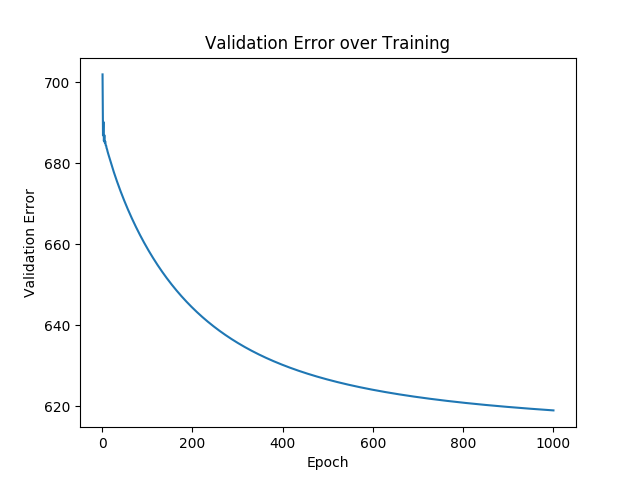
\includegraphics[width=12cm]{assets/hw_04_lr_cost.png}
  \caption{Validation Error over 1000 Epochs}
\end{figure}
The best validation error obtained by the linear regression classifier was
31.2\% after 1000 epochs. On the testing data, this classifier performed with a
70.3\% accuracy.

\subsection*{Neural Network Classifier}
For the neural network, one hidden layer was used with 16 nodes in the hidden
layer. During each epoch, the weights were adjusted to:
\begin{align*}
  W_{(1)t+1} &= W_{(1)t}-\eta Z^T\cdot(pY-Y) \\
  \diff{Z} &= (pY-Y)\cdot (W_2)^T\cdot(1-Z^2) \\
  W_{(2)t+1} &= W_{(2)t}-\eta X^T\cdot\diff{Z}
\end{align*}
\begin{figure}[H]
  \centering
  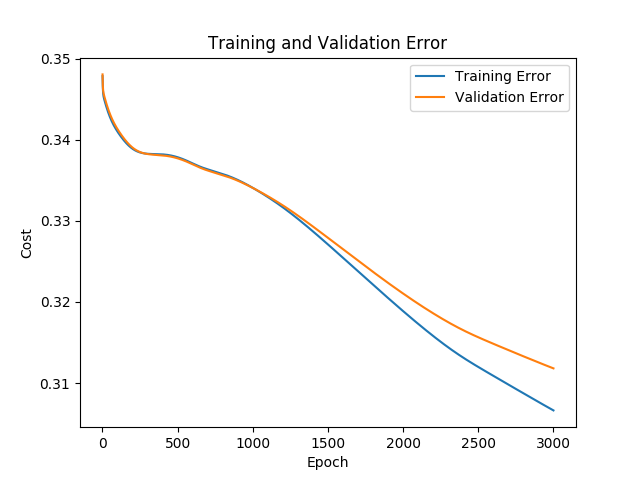
\includegraphics[width=12cm]{assets/hw_04_nn_cost_unregularized.png}
  \caption{Training and Validation Error over 3000 Epochs}
\end{figure}
The lowest validation error encountered by the neural network was 31.1\% after
3000 epochs of training. Without regularization, this neural network performed
with 67.1\% accuracy.

\subsubsection*{Regularization}
I used a regularization term equal to the following:
\[ \frac{\lambda}{2}
  \left(\sum_{i}\|W_{1(i)}\|^2+\sum_{j}\|W_{2(j)}\|^2\right) \]
\begin{figure}[H]
  \centering
  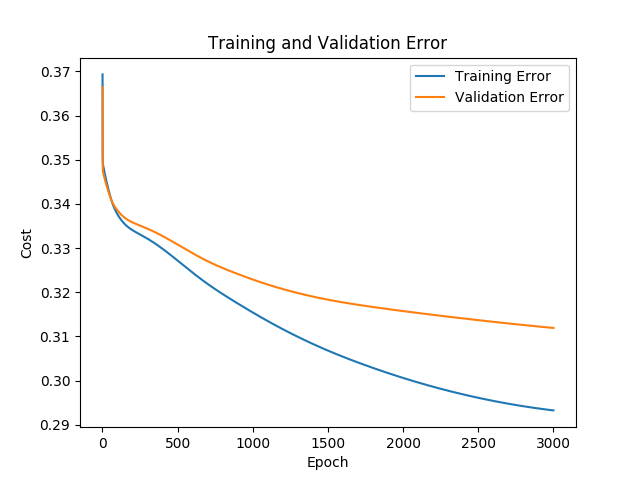
\includegraphics[width=12cm]{assets/hw_04_nn_regularized.png}
  \caption{Training and Validation Error over 3000 Epochs}
\end{figure}
After 3000 epochs, the training and validation error began to diverge, and the
lowest validation error obtained was 31.1\%. On the testing data, this neural
network performed with a 70.1\% accuracy.

\subsection*{Scikit-Learn Classifiers}
Using the support vector machine and AdaBoost ensemble classifiers provided by
\texttt{scikit-learn} gave the following results.
\begin{center}
  \begin{tabular}{|c|c|}
    \hline
    Classifier & Accuracy \\
    \hline
    SVM & 70.3\% \\
    Adaboost Ensemble & 68.5\% \\
    \hline
  \end{tabular}
\end{center}

\begin{center}
  If you have any questions, comments, or concerns, please contact me at
  alvin@omgimanerd.tech
\end{center}

\end{document}
